\documentclass[14pt, a4paper]{extarticle}
\usepackage{GOST}
\usepackage{array}
\usepackage{verbatim}
\usepackage[detect-all]{siunitx}
\usepackage{amsmath}
\usepackage{amssymb}
\usepackage[utf8]{inputenc}
\usepackage{hyperref}

\usepackage{ifthen}


\usepackage{tempora}


\makeatletter
\renewcommand\@biblabel[1]{#1.}
\makeatother

% Для листинга кода:
\usepackage{listings}
\lstset{ %
	language=python,                 % выбор языка для подсветки (здесь это С)
	basicstyle=\small\sffamily, % размер и начертание шрифта для подсветки кода
	numbers=left,               % где поставить нумерацию строк (слева\справа)
	numberstyle=\tiny,           % размер шрифта для номеров строк
	stepnumber=1,                   % размер шага между двумя номерами строк
	numbersep=5pt,                % как далеко отстоят номера строк от подсвечиваемого кода
	showspaces=false,            % показывать или нет пробелы специальными отступами
	showstringspaces=false,      % показывать или нет пробелы в строках
	showtabs=false,             % показывать или нет табуляцию в строках
	frame=single,              % рисовать рамку вокруг кода
	tabsize=2,                 % размер табуляции по умолчанию равен 2 пробелам
	captionpos=t,              % позиция заголовка вверху [t] или внизу [b] 
	breaklines=true,           % автоматически переносить строки (да\нет)
	breakatwhitespace=false, % переносить строки только если есть пробел
	escapeinside={\#*}{*)}   % если нужно добавить комментарии в коде
}


%для графиков
\usepackage{pgfplots}
\usepackage{filecontents}
\usetikzlibrary{datavisualization}
\usetikzlibrary{datavisualization.formats.functions}

\begin{document}
	
	\begin{table}[ht]
		\centering
		\begin{tabular}{|c|p{400pt}|} 
			\hline
			\begin{tabular}[c]{@{}c@{}} 
\includegraphics[scale=1]{baum.jpg} \\\end{tabular} &
			\footnotesize\begin{tabular}[c]{@{}c@{}}\textbf{Министерство~науки~и~высшего~образования~Российской~Федерации}\\\textbf{Федеральное~государственное~бюджетное~образовательное~учреждение}\\\textbf{~высшего~образования}\\\textbf{«Московский~государственный~технический~университет}\\\textbf{имени~Н.Э.~Баумана}\\\textbf{(национальный~исследовательский~университет)»}\\\textbf{(МГТУ~им.~Н.Э.~Баумана)}\\\end{tabular}  \\
			\hline
		\end{tabular}
	\end{table}
	\noindent\rule{\textwidth}{4pt}
	\noindent\rule[14pt]{\textwidth}{1pt}
	\hfill 
	\noindent
	\makebox{ФАКУЛЬТЕТ~}%
	\makebox[\textwidth][l]{\underline{~«Информатика и системы управления»~~~~~~~~~~~~~~~~~~~~~~~~~~~~~~~~~}}%
	\\
	\noindent
	\makebox{КАФЕДРА~}%
	\makebox[\textwidth][l]{\underline{~«Программное обеспечение ЭВМ и информационные технологии»~}}%
	
	
	\begin{center}
		\vspace{1.5cm}
		{\bf\huge Отчёт\par}
		{\bf\Large по лабораторной работе № 2\par}
		\vspace{0.7cm}
	\end{center}
	
	
	\noindent
	\makebox{\large{\bf Название:}~~~}
	\makebox[\textwidth][l]{\large\underline{~Программно-алгоритмическая реализация метода~}}\\
	\makebox[\textwidth][l]{\large\underline{~Рунге-Кутта 4го порядка точности при решении системы ОДУ~}}\\
	\makebox[\textwidth][l]{\large\underline{~в задаче Коши.~}}
	
	\noindent
	\makebox{\large{\bf Дисциплина:}~~~}
	\makebox[\textwidth][l]{\large\underline{~Моделирование~~~~~~~~~~~~~~~~~~~~~~~~~~}}\\
	
	\vspace{1.5cm}
	\noindent
	\begin{tabular}{l c c c c c}
		Студент      & ~ИУ7-65Б~               & \hspace{2.5cm} & \hspace{2cm}                 & &  Д.В. 
		Сусликов \\\cline{2-2}\cline{4-4} \cline{6-6} 
		\hspace{3cm} & {\footnotesize(Группа)} &                & {\footnotesize(Подпись, дата)} & & {\footnotesize(И.О. Фамилия)}
	\end{tabular}
	
	\noindent
	\begin{tabular}{l c c c c}
		Преподаватель & \hspace{5cm}   & \hspace{2cm}                 & & ~~~~~~В.М. Градов~~~~~~\\\cline{3-3} \cline{5-5} 
		\hspace{3cm}  &                & {\footnotesize(Подпись, дата)} & & {\footnotesize(И.О. Фамилия)}
	\end{tabular}
	
	\vspace{0.6cm}
	\begin{center}	
		\vfill
		\large \textit {Москва, 2021}
	\end{center}
	
	\thispagestyle {empty}
	\pagebreak
	
	% СОДЕРЖАНИЕ 
	\clearpage
		
	% ВВЕДЕНИЕ
	\clearpage
	\section*{Введение}
	\addcontentsline{toc}{section}{Введение}
	\textbf{Цель работы:} Получение навыков разработки алгоритмов решения задачи Коши при реализации моделей, построенных на системе ОДУ, с использованием метода Рунге-Кутта 4-го порядка точности.\par
	
	\textbf{Исходные данные:} Задана  система  электротехнических  уравнений,  описывающих  разрядный  контур, включающий постоянное активное сопротивление $R_k$, нелинейное сопротивление $R_p(I)$, зависящее от тока $I$, индуктивность $L_k$ и емкость $C_k$.\par
	
	
	
	\begin{equation*}
		\begin{cases}
			\frac{dI}{dT} = \frac{U - (R_k + R_p(I))I}{L_k} \\
			\frac{dU}{dt} = - \frac{I}{C_k}\\
		\end{cases}
	\end{equation*}
	Начальные условия: $t = 0, I = I_0, U = U_0$.\\
	Здесь $I, U$ - ток и напряжение на конденсаторе.\\
	Сопротивление $R_p$ рассчитать по формуле
	\begin{equation*}
		R_p = \frac{l_p}{2 \pi R^2 \int_{0}^{1}\sigma(T(z))zdz}
	\end{equation*}
	Для функции $T(z)$ применить выражение $T(z) = T_0 + (T_w - T_0)z^m$.\\
	Параметры $T_0$, $m$ находятся интерполяцией из табл.1 при известном токе I.\\
	Коэффициент электропроводности $\sigma(T)$ зависит от $T$ и рассчитывается интерполяцией из табл.2.\par
	\newpage
	Таблица 1\par
	\begin{table}[h]
		\begin{tabular}{|l|l|l|}\hline
			$I, A$    & $T_0, K$  & $m$\\ \hline
			0.5 & 6730  & 0.50 \\
			1 & 6790  & 0.55 \\
			5 & 7150  & 1.7 \\
			10 & 7270  & 3 \\
			50 & 8010  & 11\\
			200 & 9185  & 32 \\
			400 & 10010  & 40 \\
			800 & 11140  & 41 \\
			1200 & 12010  & 39 \\
			\hline     
		\end{tabular}
	\end{table}\par
	
	Таблица 2\par
	\begin{table}[h!]
		\begin{tabular}{|l|l|}\hline
			$T, K$    & $\sigma, 1/\text{Ом см}$ \\ \hline
			4000 & 0.031 \\
			5000 & 0.27 \\
			6000 & 2.05 \\
			7000 & 6.06 \\
			8000 & 12.0 \\
			9000 & 19.9 \\
			10000 & 29.6 \\
			11000 & 41.1 \\
			12000 & 54.1 \\
			13000 & 67.7 \\
			14000 & 81.5 \\
			\hline     
		\end{tabular}
	\end{table}\par
	\newpage
	Параметры разрядного контура:
	\noindent$
	R = 0.35\text{ см},\\
	L_e = 12\text{ см},\\
	L_k = 187 * 10^{-6}\text{ Гн},\\
	C_k = 268 * 10^{-6}\text{ Ф},\\
	R_k = 0.25\text{ Ом},\\
	U_c = 1400\text{ В},\\
	I_0 = 0..3\text{ А},\\
	T_w = 2000\text{ К}
	$\par
	
	\textbf{Теоритические сведения:}\\
	Метод Рунге-Кутты 4-го порядка точности.
	
	
	\begin{equation*}
		y_{n+1} = y_n + \frac{k_1 + 2k_2 + 2k_3 + k_4}{6},
	\end{equation*}
	
	\begin{equation*}
		z_{n+1} = z_n + \frac{q_1 + 2q_2 + 2q_3 + q_4}{6}
	\end{equation*}
	
	\begin{equation*}
		k_1 = h_n f(y_n, z_n), ~~q_1 = h_n \varphi (y_n)
	\end{equation*}
	
	\begin{equation*}
		k_2 = h_n f (y_n + \frac{k_1}{2}, z_n + \frac{q_1}{2}),~~ q_2 = h_n \varphi(y_n + \frac{k_1}{2})
	\end{equation*}
	
	\begin{equation*}
		k_3 = h_n f (y_n + \frac{k_2}{2}, z_n + \frac{q_2}{2}), ~~q_3 = h_n \varphi(y_n + \frac{k_2}{2})
	\end{equation*}
	
	\begin{equation*}
		k_4 = h_n f (y_n + k_3, z_n + q_3, ~~q_4 = h_n \varphi(y_n + k_3)
	\end{equation*}
	
	\newpage
	\textbf{Результат работы}
	\begin{enumerate}
		\item Графики зависимости от времени импульса t: $I(t),U(t),R_p(t),$ произведения $I(t)R_p(t), T_0(t)$ при заданных выше параметрах. Указать шаг сетки.\\
		\begin{figure}[h]
			\centering
			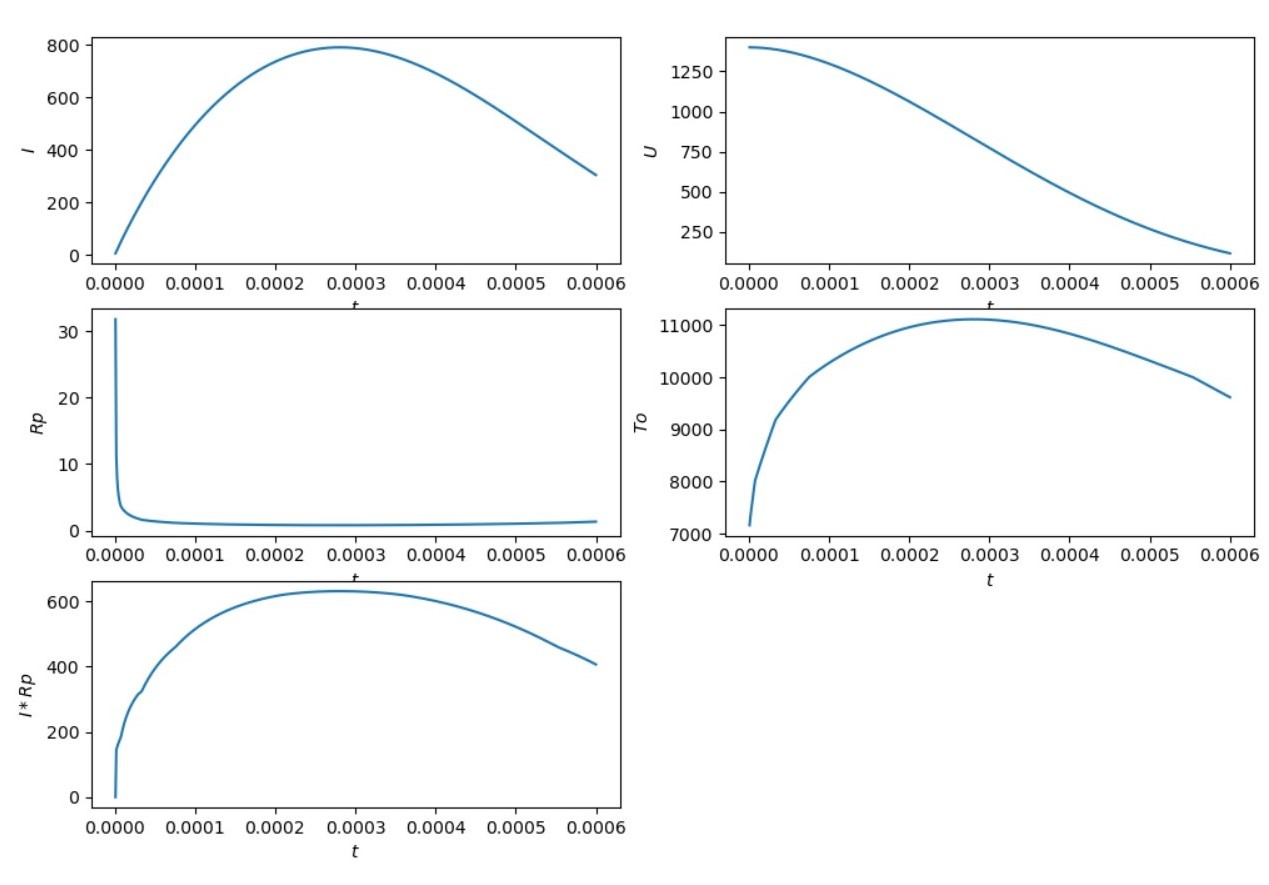
\includegraphics[scale=0.65]{graphics/graphs1.jpg}
		\end{figure}\par
		Шаг  - $10^{-6}$
		\newpage
		
		\item График зависимости $I(t)$ при $R_k+R_p=0$. Обратить внимание на то, что в этом случае колебания тока будут незатухающими.\\
		\begin{figure}[h]
			\centering
			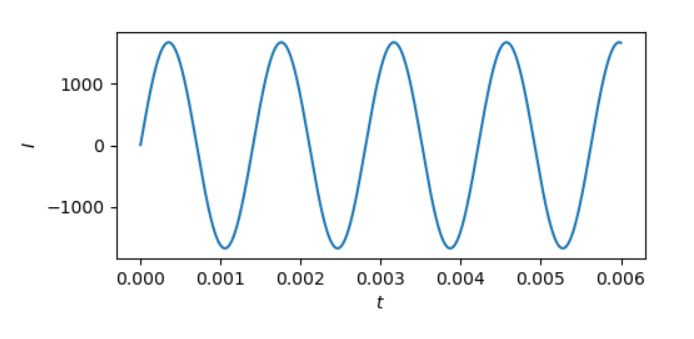
\includegraphics[scale=1]{graphics/graphs2.jpg}
		\end{figure}\par
		
		\item График зависимости $I(t)$ при $R_k + R_p = \text{const} = 200$ Ом в интервале значений 0 - 20 мкс.
		\begin{figure}[h]
			\centering
			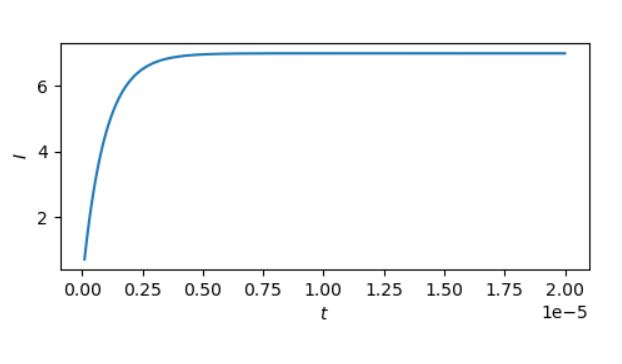
\includegraphics[scale=1]{graphics/graphs3.jpg}
		\end{figure}\par
		
		\item Результаты исследования влияния параметров контура $C_k, L_k, R_k$ на длительность импульса $t_{\text{имп}}$ апериодической формы. Длительность импульса определяется по кривой зависимости тока от времени на высоте $0.35I_{\text{max}}, I_{\text{max}}$ - значение тока в максимуме.\\
		\newpage
		График при начальных значениях:
		\begin{figure}[h!]
			\centering
			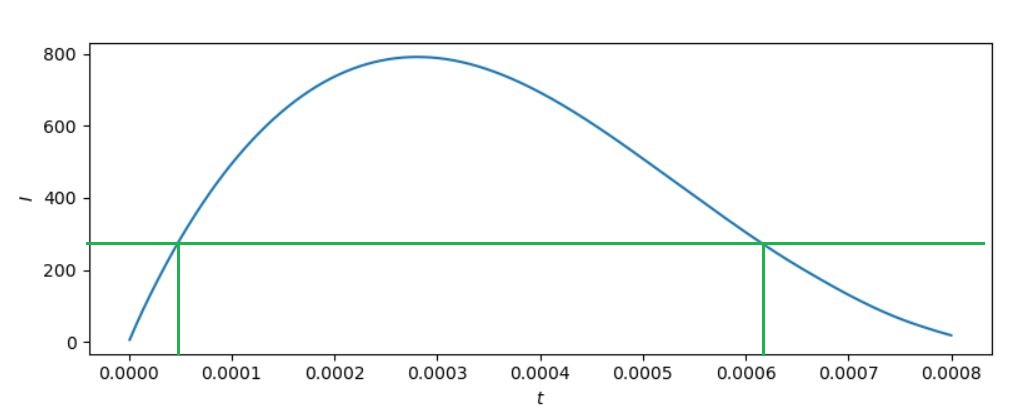
\includegraphics[scale=0.8]{graphics/graphs41.jpg}
		\end{figure}\par
		Длительность импульса чуть меньше 6 мкс.
		
		График при увеличении $C_k$ в 2 раза:
		\begin{figure}[h!]
			\centering
			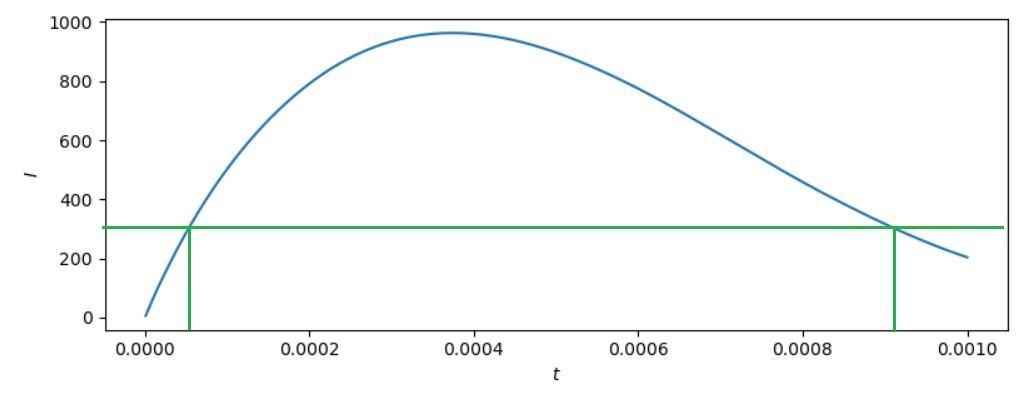
\includegraphics[scale=0.8]{graphics/graphs43.jpg}
		\end{figure}\par
		Длительность импульса около 9 мкс. \\
		При увеличении $C_k$, $t_{\text{имп}}$ увеличивается.
		\newpage
		График при уменьшении $C_k$ в 2 раза:
		\begin{figure}[h]
			\centering
			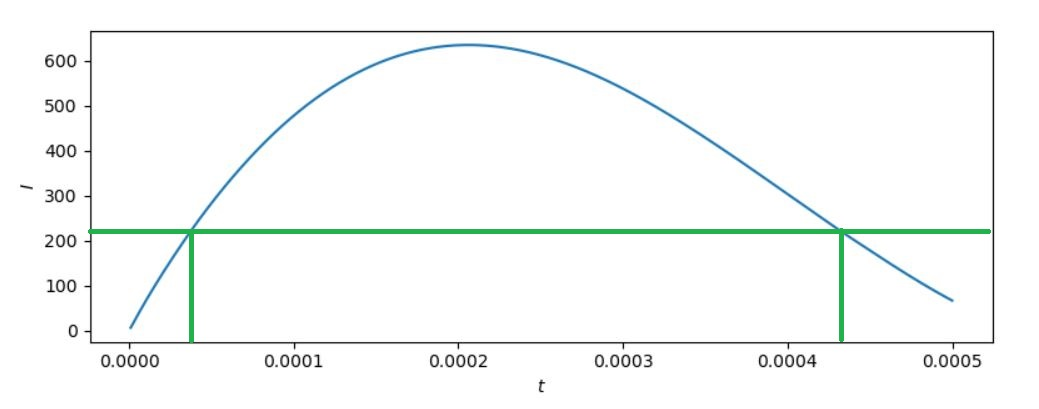
\includegraphics[scale=0.8]{graphics/graphs45.jpg}
		\end{figure}\par
		Длительность импульса около 4 мкс. \\
		При уменьшении $C_k$, $t_{\text{имп}}$ уменьшается.\par
		Можно сделать вывод, что $C_k$, $t_{\text{имп}}$ пропорционально зависимы.
		\newpage 
				
		График при увеличении $L_k$ в 2 раза:
		\begin{figure}[h]
			\centering
			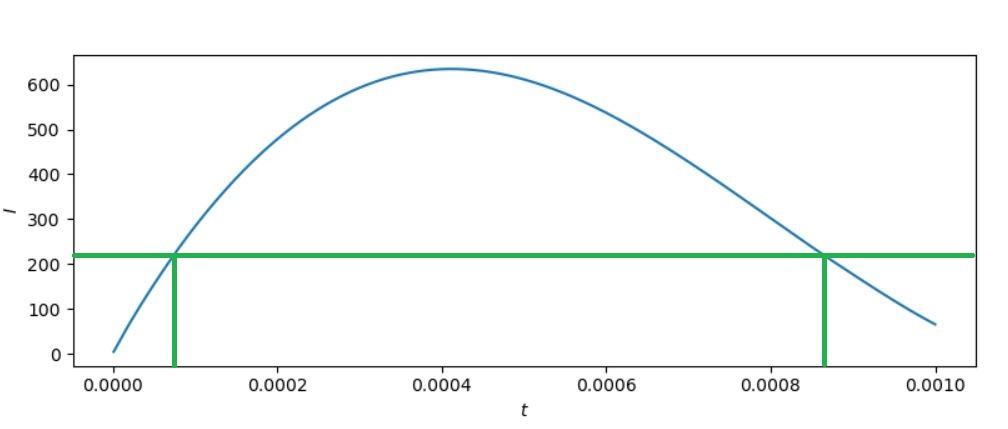
\includegraphics[scale=0.8]{graphics/graphs47.jpg}
		\end{figure}\par
		Длительность импульса около 8 мкс.\\
		При увеличении $L_k$, $t_{\text{имп}}$ увеличивается.
		
		График при уменьшении $L_k$ в 2 раза:
		\begin{figure}[h]
			\centering
			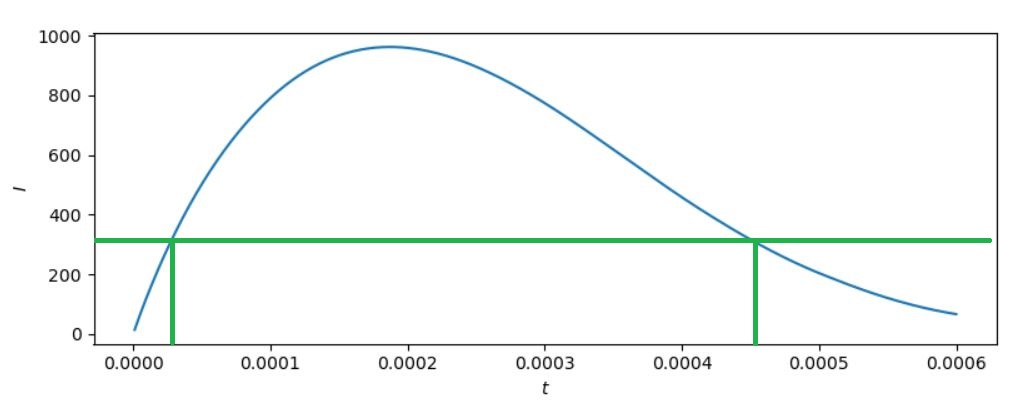
\includegraphics[scale=0.8]{graphics/graphs49.jpg}
		\end{figure}\par
		Длительность импульса около 4 мкс.\\
		При уменьшении $L_k$, $t_{\text{имп}}$ уменьшается.\par
		Можно сделать вывод, что $L_k$, $t_{\text{имп}}$ пропорционально зависимы.
		\newpage 
		
		График при увеличении $R_k$ в 5 раза:
		\begin{figure}[h]
			\centering
			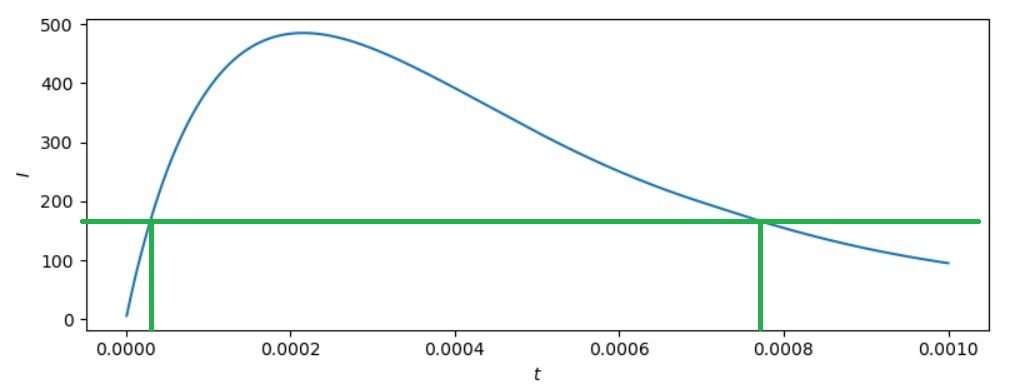
\includegraphics[scale=0.8]{graphics/graphs411.jpg}
		\end{figure}\par
		Длительность импульса чуть меньше 8 мкс.
		При увеличении $R_k$, $t_{\text{имп}}$ увеличивается.

		График при уменьшении $R_k$ в 5 раза:
		\begin{figure}[h]
			\centering
			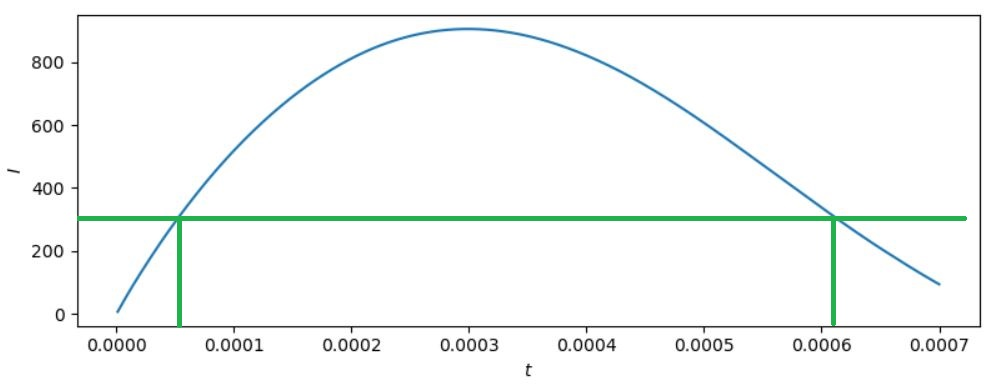
\includegraphics[scale=0.8]{graphics/graphs413.jpg}
		\end{figure}\par
		При уменьшении $R_k$, $t_{\text{имп}}$ уменьшается.\par
		Можно сделать вывод, что $R_k$, $t_{\text{имп}}$ пропорционально зависимы.
		\newpage		
	\end{enumerate}
	
	\textbf{Ответы на вопросы}\par
	\begin{enumerate}
		\item Какие способы тестирования программы, кроме указанного в п.2, можете предложить ещё?\par
		Можно изменять параметры $I_0, U_{c0}, R_k$ при $R_p(I) = 0$. Если значение $R_k$ будет велико, то будет наблюдаться апериодическое затухание, при малых значениях - затухающие колебания.
		\item Получите систему разностных уравнений для решения сформулированной задачи неявным методом трапеций. Опишите алгоритм реализации полученных уравнений.\par
		$
			u_{n+1} = u_n + \int_{x_n}^{x_{n+1}}f(x, u(x)) dx\\
			u_{n+1} = u_n + \frac{h}{2}[f(x_n, y_n) + f(x_{n+1}, u_{n+1})] + O(h^2)\\ \\	
			\begin{cases}			
				\frac{dI}{dT} = \frac{U - (R_k + R_p(I))I}{L_k}\\
				\frac{dU}{dT} = \frac{- I}{C_k}
				
			\end{cases}\\ \\		
			I_{n+1} = I_n + \frac{h}{2}[\frac{U_n - (R_k + R_p(I_n))I_n}{L_k} + \frac{U_{n+1} - (R_k + R_p(I_{n+1}))I_{n+1}}{L_k}]\\
			U_{n+1} = U_n + \frac{h}{2} [-\frac{I_n}{C_k} - \frac{I_{n+1}}{C_k}] =
			U_n - \frac{h}{2}[\frac{I_n + I_{n+1}}{C_k}]\\
			\text{Подставляя $U_{n+1}$ в выражение для $I_{n+1}$}\\			
			I_{n+1} = I_n + \frac{h}{2L_k}[2U_n - (R_k + R_p(I_n) + \frac{h}{2C_k})I_n
			-(R_k + R_p(I_{n+1}) + \frac{h}{2C_k})I_{n+1}]\\
			\text{Получим уравнение вида}\\
			x = f(x)\\
		$
		Его можно решить методом простых итераций или методом Ньютона, после этого определить $U_{n+1}$.
		\newpage
		
		\item Из каких соображений проводится выбор численного метода того или
		иного порядка точности, учитывая, что чем выше порядок точности метода, тем он более сложен и требует, как правило, больших ресурсов вычислительной системы?\par
		Выбор порядка точности численного метода зависит от вида правой части дифференциального уравнения и требуемой точности вычислений.
		$\phi(x, u) \equiv \phi(x)$ \par
		Если правая часть непрерывна и ограничена, и её четвёртые производные тоже, то использование метода Рунге-Кутта четвёртого порядка имеет смысл. В противном случае предельный (четвертый) порядок схемы Рунге-Кутта не может быть достигнут, и стоит использовать более простые схемы.
  

		
		
		
	\end{enumerate}
	
	\newpage
	\textbf{Реализация}
	
	\begin{lstlisting}[caption=Интерполяция]
		def interpolate(value, table_v, table):
			end = 1
			start = 0
			i = 0
			
			while ((i < (len(table_v))) and (value > table_v[i])):
				i += 1
				end = i
			
			start = end - 1
			
			return table[start] + (table[end] - table[start]) / (table_v[end] - table_v[start]) * (value - table_v[start])
	\end{lstlisting}

	\begin{lstlisting}[caption=Интегрирование]
		def f_integr(I, z):
			t0 = interpolate(I, table_I, table_T0)
			m = interpolate(I, table_I, table_m)
			t = t0 + (tw - t0) * (z ** m)
			sigma = interpolate(t, table_T, table_sigma)
			
			return sigma * z
		
		def i_integr(I):
			a = 0
			b = 1
			n = 100
			h = (b - a) / n
			s = (f_integr(I, a) + f_integr(I, b)) / 2
			x = 0
			
			for _ in range(n - 1):
				x = x + h
				s = s + f_integr(I, x)
				s = s * h
			
			return s
	\end{lstlisting}

	\begin{lstlisting}[caption=Вычисление сопротивления Rp]
		def Rp(le, R, I):
			return le / (2 * pi * R * R * i_integr(I))
	\end{lstlisting}

	\begin{lstlisting}[caption=Решение системы уравнений методом Рунге-Кутта]	
		def f(I, U, le, R, Lk, Rk):
			global global_rp
			global_rp = Rp(le, R, fabs(I))
			return (U - (Rk + global_rp) * I) / Lk
		
		def g(I, Ck):
			return -I / Ck
		
		def runge_kutta_I_U(I, U, le, R, Lk, hn, Rk, Ck):
			k1 = f(I, U, le, R, Lk, Rk)
			q1 = g(I, Ck)
			
			k2 = f(I + hn * k1 / 2, U + hn * q1 / 2, le, R, Lk, Rk)
			q2 = g(I + hn * k1 / 2, Ck)
			
			k3 = f(I + hn * k2 / 2, U + hn * q2 / 2, le, R, Lk, Rk)
			q3 = g(I + hn * k2 / 2, Ck)
			
			k4 = f(I + hn * k3, U + hn * q3, le, R, Lk, Rk)
			q4 = g(I + hn * k3, Ck)
			
			return I + hn * (k1 + 2 * k2 + 2 * k3 + k4) / 6,\
			U + hn * (q1 + 2 * q2 + 2 * q3 + q4) / 6
	\end{lstlisting}

	
\end{document}